\documentclass[12pt, letterpaper]{scrartcl}

\usepackage{fullpage} % Set margins and place page numbers at bottom center
\usepackage[shortlabels]{enumitem} % Use a. in the enumerate
\usepackage{amsmath} % aligned equations
\usepackage{graphicx} % include figure
\usepackage{float} % usage of H for figure float
\usepackage{amssymb} % \varnothing

\begin{document}

% ### Header - start ###
    \begin{center}
    	\hrule
    	\vspace{0.4cm}
    	{\textbf { {\large Homework 1} \\ EE 513 --- Stochastic Systems Theory}}
    \end{center}
    { \textbf{Name:} Ali Zafari \hspace{\fill} \textbf{Student Number:} 800350381 \hspace{\fill} \textbf{Fall 2022} } \newline\hrule
% ### Header - end ###

\paragraph*{Problem 1.1} \hfill

\begin{enumerate}[a.]
    \item Each link in the network can have 2 states, exist or not. The sample space of the network with 4 links can be written as:\\\\
    \begin{tabular}{ c|c|c|c|c|c|c|c } 
     \textbf{\#} & 1 & 2 &3&4&5&6&7\\ \hline
     \textbf{S} & None & a&b&c&d&ab&ac \\ \hline
     \textbf{P} & $(1-p)^4$ &$p(1-p)^3$&$p(1-p)^3$&$p(1-p)^3$&$p(1-p)^3$&$p^2(1-p)^2$&$p^2(1-p)^2$\\
    \end{tabular}

    \begin{tabular}{ c|c|c|c|c|c|c } 
     8&9&10&11&12&13&14\\ \hline
     ad&bc&bd&cd&abc&abd&acd \\ \hline
     $p^2(1-p)^2$&$p^2(1-p)^2$&$p^2(1-p)^2$&$p^2(1-p)^2$&$p^3(1-p)^1$&$p^3(1-p)^1$&$p^3(1-p)^1$
    \end{tabular}
    
    \begin{tabular}{ c|c } 
     15&16\\ \hline
     bcd&abcd \\ \hline
     $p^3(1-p)^1$&$p^4$
    \end{tabular}
    
    The sigma-algebra $\mathcal{F}$ includes all the possible subsets of the sample space with their corresponding probabilities. The total number of elements covered in $\mathcal{F}$ (including the empty set, i.e., $\varnothing$) will be $2^{16}$.

    
    \item We would consider all the outcomes which result in the event that nodes 1 and 4 have a connection. To have established the connection, link $a$ must exist, then one links $d$ and $cb$ must at least exist.
    \begin{align*}
        A &= \{ad, abc, abd, acd, abcd\}
    \end{align*}
    outcomes in $A$ are mutually exclusive:
    \begin{align*}
        P(A) &= P(ad)+P(abc)+P(abd)+P(acd)+P(abcd)\\
        &= p^2(1-p)^2+p^3(1-p)^1+p^3(1-p)^1+p^3(1-p)^1+p^4\\
        &= p^2-2p^3+p^4+3p^3-3p^4+p^4\\
        &=p^2+p^3-p^4
    \end{align*}
    
    \item To have connection between nodes 2 and 3, either links $c$ or $bd$ must exist.
    \begin{equation*}
        B = \{c, ac, bc, cd, bd, abc, abd, acd, bcd, abcd\}
    \end{equation*}
    outcomes in $B$ are mutually exclusive:
    \begin{align*}
    \begin{split}
       P(B) &= P(c)+P(ac)+P(bc)+P(cd)+P(bd)\\
       &\quad +P(abc)+P(abd)+P(acd)+P(bcd)+P(abcd)
    \end{split}\\
    \begin{split}
        &= p(1-p)^3+4\times p^2(1-p)^2+4\times p^3(1-p)^1+p^4\\
        &= p+p^2-p^3 
    \end{split}
    \end{align*}
    \item 
    \begin{equation*}
        A\cap B=\{abc, acd, abd, abcd\}
    \end{equation*}
    outcomes in $A\cap B$ are mutually exclusive:
    \begin{align*}
        P(A\cap B) &= P(abc)+P(acd)+P(abd)+P(abcd)\\
        &= 3\times p^3(1-p)^1+p^4\\
        &= 3p^3-2p^4
    \end{align*}
    To check if two events $A$ and $B$ are independent or not, we calculate $P(A)\times P(B)$:
    \begin{align*}
        P(A)P(B) &= (p^2+p^3-p^4)(p+p^2-p^3)\\
        &= p^3+p^4-p^5+p^4+p^5-p^6-p^5-p^6+p^7\\
        &= p^3+2p^4-p^5-2p^6+p^7\\
        &\neq P(A\cap B)
    \end{align*}
    Therefore $A$ and $B$ are not independent.
    
    \item Availability of $c$ partitions the sample space, i.e., $S=C\cup\bar{C}$ therefore:
    \begin{align*}
        P(A)&=P(A\cap S)\\
        &=P(A\cap(C\cup\bar{C}))\\
        &=P((A\cap C)\cup (A\cap\bar{C}))  \qquad \text{[mutually exclusive]}\\
        &=P(A\cap C) + P(A\cap\bar{C}) \qquad \text{[Bayes rule]}\\
        &=P(C)P(A|C)+P(\bar{C})P(A|\bar{C})\\
        &=pP(A|C)+(1-p)P(A|\bar{C})\\
        &=p(2p^2(1-p)+p^3) + (1-p)(p^2(1-p)+p^3)\\
        &=2p^3-p^4+p^2-p^3\\
        &=p^2+p^3-p^4
    \end{align*}
    \item By moving the link c in-between nodes 1 and 2, the event $A_{new}$ (nodes 1 and 4 can communicate) have outcomes as follows:
    \begin{align*}
        A_{new} &= \{ad, cd, abd, acd, cbd, abcd\}
    \end{align*}
    outcomes in $A_{new}$ are mutually exclusive:
    \begin{align*}
        P(A_{new}) &= P(ad)+P(cd)+P(abd)+P(acd)+P(cbd)+P(abcd)\\
        &= 2\times p^2(1-p)^2+3\times p^3(1-p)^1+p^4\\
        &= 2p^2-4p^3+2p^4+3p^3-3p^4+p^4\\
        &= 2p^2-p^3
    \end{align*}
    To verify $P(A_{new})>^?P(A)$, we calculate their difference:
    \begin{align*}
        P(A_{new})-P(A)&=2p^2-p^3 - (p^2+p^3-p^4)\\
        &=p^2-2p^3+p^4\\
        &=p^2(1-2p+p^2)\\
        &=p^2(1-p)^2
    \end{align*}
    $p^2(1-p)^2$ is always greater than zero, therefore $P(A_{new})>P(A)$.
\end{enumerate}
\hrule

\paragraph*{Problem 1.2} \hfill\\
We assume that $x$ divides the unit length stick at random ($x\in[0,1]$), then $y$ is chosen to be less than $x$ ($0<y<x$) as depicted in Figure \ref{fig:stick}. This assumption makes the sample space as shown in Figure \ref{fig:space} (solid lines). 
\begin{figure}[H]
    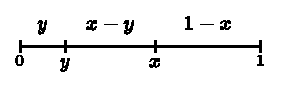
\includegraphics[width=0.3\linewidth]{hw1_figures/p1.2a.pdf}
    \centering
    \caption{stick of unit length}
    \label{fig:stick}
\end{figure}
For the 3 dividened lengths to create a triangle, all 3 triangle inequalities must be satisfied simultaneously:
    \begin{enumerate}[i.]
        \item
        \begin{align*}
            y+x-y>1-x \quad \longrightarrow \quad x>0.5
        \end{align*}
        \item
        \begin{align*}
            y+1-x>x-y \quad \longrightarrow \quad 2y-2x+1>0
        \end{align*}
        \item
        \begin{align*}
            x-y+1-x>y \quad \longrightarrow \quad y<0.5
        \end{align*}
    \end{enumerate}
\begin{figure}[H]
    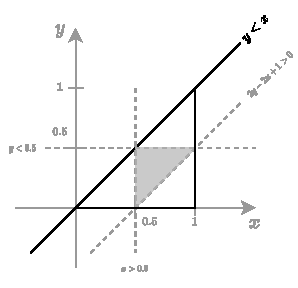
\includegraphics[width=0.5\linewidth]{hw1_figures/p1.2.pdf}
    \centering
    \caption{Sample space (solid lines) and target event (shaded area)}
    \label{fig:space}
\end{figure}
So we can calculate the probability based on the ratio of area of the event and area of the sample space:
\begin{align*}
    P(triangle)=\frac{\frac{1}{2}\times\frac{1}{2}\times\frac{1}{2}}{\frac{1}{2}\times1\times1}=\frac{1}{4}=0.25
\end{align*}
\hrule
\paragraph*{Problem 1.3} \hfill\\
Probability of intersection of events $A_n$ and $B_m$ can be written in terms of conditional probabilities using the product rule:
\begin{align*}
    P(A_n\cap B_m)&=P(A_n)P(B_m|A_n)\\
    &=P(B_m)P(A_n|B_m)
\end{align*}
so by re-arranging, we have:
\begin{align*}
    P(B_m|A_n)=\frac{P(A_n|B_m)P(B_m)}{P(A_n)}
    \tag{$*$}
    \label{eq:bayes}
\end{align*}
As $B_i$'s partition the sample space, we have $\bigcup_{i=1}^MB_i=S$. So we can conclude:
\begin{align*}
    P(A_n)&=P(A_n\cap S)\\
    &=P(A_n\cap (\bigcup_{i=1}^MB_i))\\
    &=P(\bigcup_{i=1}^M(A_n\cap B_i)) \qquad \text{[mutually exclusive]}\\
    &=\sum_{i=1}^MP(A_n\cap B_i)\qquad \text{[conditional probability]}\\
    &=\sum_{i=1}^MP(A_n|B_i)P(B_i)
    \tag{$\dagger$}
    \label{eq:evidence}
\end{align*}
Now we only need to replace (\ref{eq:evidence}) in equation (\ref{eq:bayes}) to have:
\begin{align*}
    P(B_m|A_n)=\frac{P(A_n|B_m)P(B_m)}{\sum_{i=1}^MP(A_n|B_i)P(B_i)}
\end{align*}
\hrule

\paragraph*{Problem 1.4} \hfill
\begin{enumerate}[a.]
    \item With the law of total probability:\\
    \begin{align*}
        P(out=0)&=P(out=0 \cap in=0) + P(out=0 \cap in=1)\\
        &=P(out=0|in=0)P(in=0)+P(out=0|in=1)P(in=1)\\
        &=(1-\epsilon)\times0.4 + 0\times0.6\\
        &=0.4(1-\epsilon)
    \end{align*}
    \begin{align*}
        P(out=1)&=P(out=1 \cap in=0) + P(out=1 \cap in=1)\\
        &=P(out=1|in=0)P(in=0)+P(out=1|in=1)P(in=1)\\
        &= 0\times0.4+(1-\epsilon)\times0.6\\
        &=0.6(1-\epsilon)
    \end{align*}
    \begin{align*}
        P(out=erasure)&=P(out=erasure \cap in=0) + P(out=erasure \cap in=1)\\
        &=P(out=erasure|in=0)P(in=0)+P(out=erasure|in=1)P(in=1)\\
        &= \epsilon\times0.4+\epsilon\times0.6\\
        &=\epsilon
    \end{align*}
    \item Probability of input being $0$ given output is $1$, utilizing Bayes rule:
    \begin{align*}
        P(in=0|out=1)&=\frac{P(out=1|in=0)P(in=0)}{P(out=1)}\\
        &=\frac{0\times 0.4}{0.6(1-\epsilon)}=0
    \end{align*}
    
    Probability of input being $1$ given output is $1$, utilizing Bayes rule:
    \begin{align*}
        P(in=1|out=1)&=\frac{P(out=1|in=1)P(in=1)}{P(out=1)}\\
        &=\frac{(1-\epsilon)\times 0.6}{0.6(1-\epsilon)}=1
    \end{align*}
\end{enumerate}
\hrule
\paragraph*{Problem 1.5} \hfill
\begin{enumerate}[a.]
    \item Sample space of received signal $Y$ from the transmitted signal $X$ written as tuples of $(x,y)$:
    \begin{align*}
        S_{(x,y)}=\{(-2,-2), (-2,-1), (-2,0), (+2,0), (+2,+1), (+2,+2)\}
    \end{align*}
    \item 
    \begin{align*}
        \{\text{X is definitely +2} \}_{(x,y)}=\{(+2,+1), (+2,+2)\}
    \end{align*}
    \item
    To have outcome $Y=0$, two different situations can be hypothesized to cover the corresponding outcomes in the sample space, i.e., $\{(-2,0), (+2,0)\}$
    \begin{enumerate}[i.]
        \item Transmitted signal was $-2$ and the numbers of head in 2 tosses of the coin is 2. 
        \item Transmitted signal was $+2$ and the numbers of head in 2 tosses of the coin is 2.
    \end{enumerate} 
\end{enumerate}
\hrule

\paragraph*{Problem 1.6} \hfill
\begin{enumerate}[a.]
    \item The probability distribution is a binomial with $N=100$ and $p=10^{-2}$:
    \begin{align*}
        P(\text{block accepted})&=P(\text{2 or fewer errors in the received block})\\
        &=P(\text{no error})+P(\text{1 bit error})+P(\text{2 bits error})\\
        &= {100\choose0}(0.01)^0(0.99)^{100}+{100\choose1}(0.01)^1(0.99)^{99}+{100\choose2}(0.01)^2(0.99)^{98}\\
        &=0.9206
    \end{align*}
    \item The re-transmit probability is:
    \begin{align*}
        P(\text{Re-transmit})&=P(\text{more than 2 errors in the received block})\\
        &=1-P(\text{2 or fewer errors in the received block})\\
        &= 1-0.9206=0.0794
    \end{align*}
    To have $M$ re-transmissions, the block should be accepted at the $(M+1)^{th}$ transmission, so the probability will be:
    \begin{align*}
        P(\text{M-Retransmissions})&=P(\text{Re-transmit})^M\times P(\text{block accepted at }(M+1)^{th})\\
        &=(0.0794)^M(0.9206)
    \end{align*}
\end{enumerate}
\hrule
\end{document}

